
\setcounter{figure}{0}
\renewcommand{\thefigure}{8.\arabic{figure}}
\section{GUI}
 We designed an application that provides a graphical user interface (GUI) designed to facilitate the translation to Braille text from images, with additional features for generating speech output. This document outlines the components and functionality of the GUI, emphasizing its accessibility for visually impaired users. The application is built to run on both Windows 10 and Windows 11. However, it can be adjusted to be built on Linux as well.

\subsection{Design Features}


\begin{itemize}
    \item \textbf{Central Widget}: This widget serves as the main container for the GUI elements.
    
    \item \textbf{Stacked Widget}: Used to manage different pages within the GUI.
    
    \begin{itemize}
        \item \textbf{Page 1 - Initial Translation Options:}: The initial screen allows users to select their translation options, such as translating multiple images, a single image, or enabling speech generation.

        \begin{figure}[h!]
            \centering
            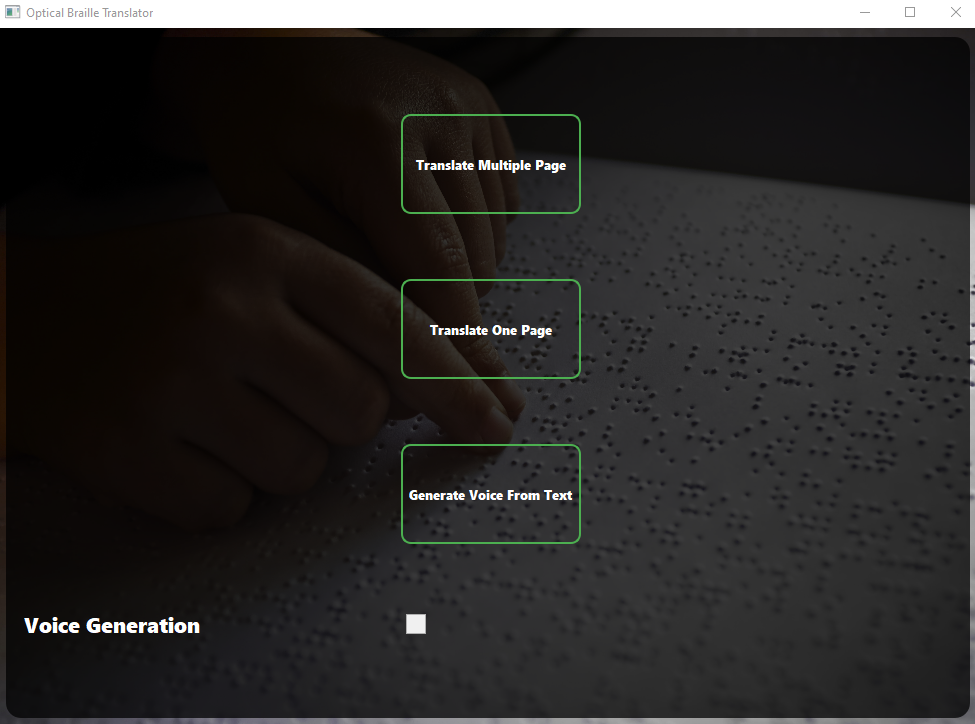
\includegraphics[width=0.6\textwidth]{main_page.png}
            \caption{Design layout of Page 1 - Initial Translation Options}
        \end{figure}
        
        \begin{itemize}
            \item \textbf{Translate Multiple Pages}: Button to initiate translation of multiple images.
            \item \textbf{Translate One Page}: Button to translate a single image.
            \item \textbf{Voice Generation}: Checkbox for enabling Speech generation.
            \item \textbf{Generate Voice From Text}: Button to generate Speech from translated text.
        \end{itemize}
        
        \item \textbf{Page 2 - Configuration Settings:}: This screen is used for configuring the translation settings, including selecting the type of translation, enabling image processing, choosing AI-based translation, and browsing input files or folders.

        \begin{figure}[h!]
            \centering
            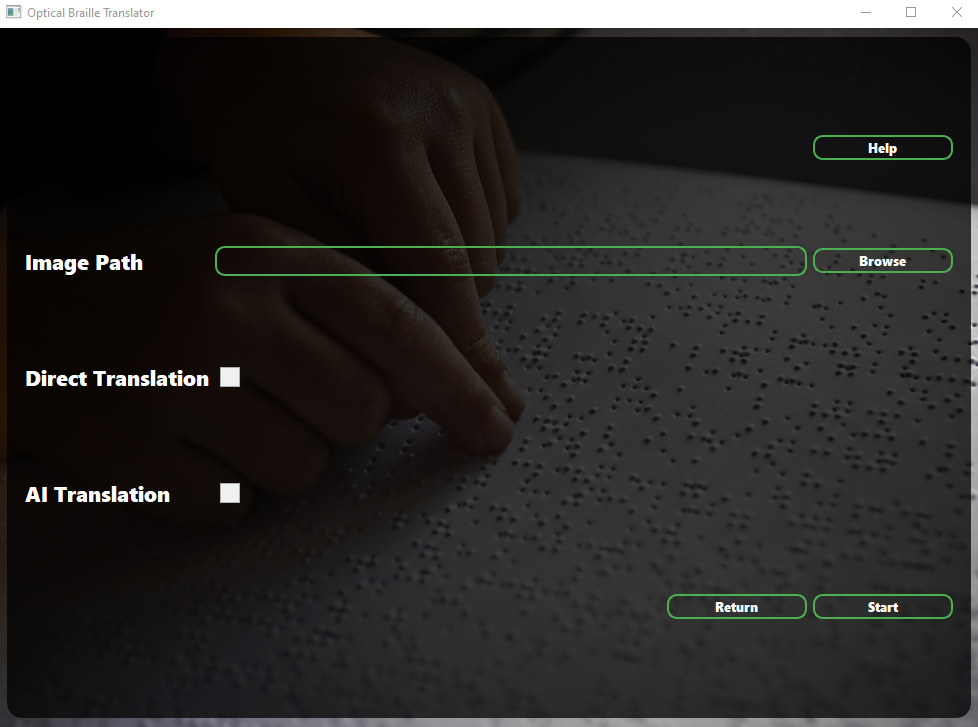
\includegraphics[width=0.6\textwidth]{options_page.png}
            \caption{Design layout of Page 2 - Configuration Settings}
        \end{figure}
        
        \begin{itemize}
            \item \textbf{Direct Translation}: Checkbox for selecting image processing mode.
            \item \textbf{AI Translation}: Checkbox for selecting AI-based translation.
            \item \textbf{Browse}: Button to browse and select input files or folders.
            \item \textbf{Path Label}: Label displaying the selected file or folder path.
            \item \textbf{Return Button}: Button to return to the home screen.
            \item \textbf{Start Button}: Button to start the translation process.
        \end{itemize}
        
        \item \textbf{Page 3 - Audio Playback and Text Display:}: This screen is designed for text display, allowing users to pen generated text and audio files, and view the translated text.

        \begin{figure}[h!]
            \centering
            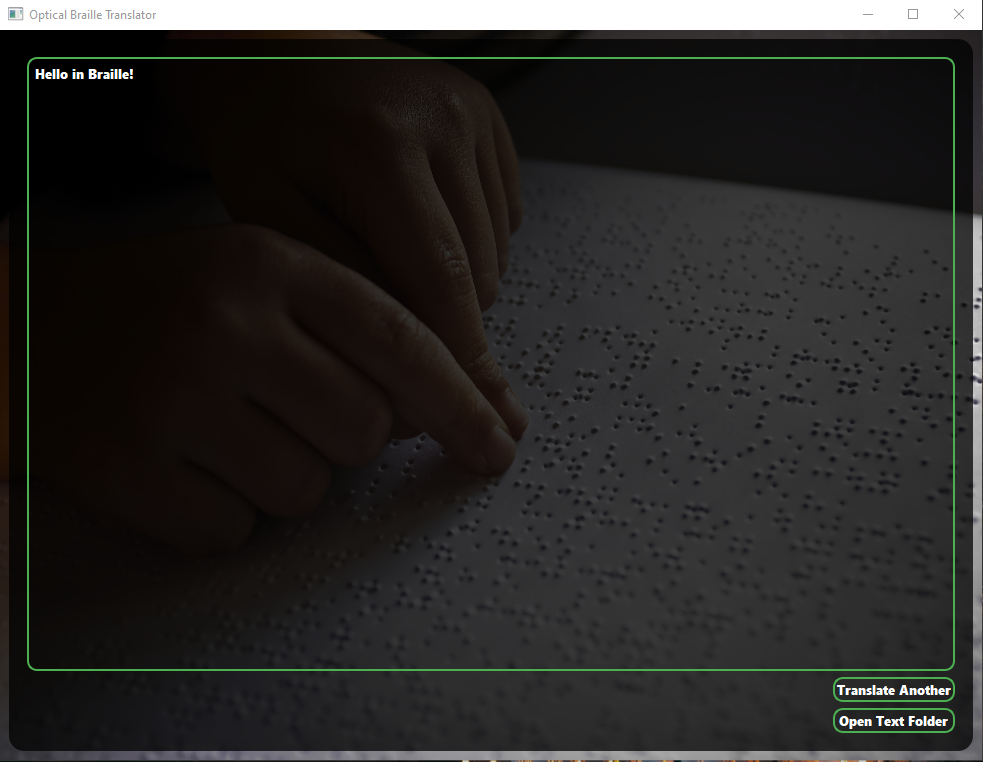
\includegraphics[width=0.6\textwidth]{result_page.png}
            \caption{Design layout of Page 3 - Text Display}
        \end{figure}
        
        \begin{itemize}
            \item \textbf{Open Translation Results Folder Button}: Button to open the folder containing generated text files and speech audio.
            \item \textbf{Text Display}: Text browser widget to display translated and corrected text.
            \item \textbf{Translate Another}: To translate a new file. This button returns the user back to the main page.
        \end{itemize}
    \end{itemize}
\end{itemize}

\subsection{Tools and Frameworks}
The development of the Optical Braille Translator application GUI leverages various tools and frameworks to ensure efficiency and reliability. Key tools and frameworks include:

\begin{itemize}
    \item \textbf{Qt Designer}: Utilized for creating the graphical user interface with a focus on cross-platform compatibility.
    \item \textbf{OpenCV}: Employed for image processing tasks to detect and translate Braille text from images.
    \item \textbf{TensorFlow}: Used for AI-based translation capabilities, enhancing the accuracy of Braille text recognition.
    \item \textbf{PyQt}: Provides the integration of Python with Qt, facilitating the development of the application in Python. The version used is PyQt5.
\end{itemize}


\subsection{Accessibility Features}

The GUI of the Optical Braille Translator application is designed to be accessible for visually impaired users, adhering to accessibility standards and providing the following features:

\begin{itemize}
    \item \textbf{High Contrast and Custom Styling}: Utilizes high contrast colors and custom styling for improved readability and navigation.
    
    \item \textbf{Text-to-Speech (TTS) Integration}: Enables speech generation from translated text, supporting users who rely on auditory feedback.
    
    \item \textbf{Keyboard Navigation and Screen Reader Compatibility}: Supports keyboard navigation and is compatible with screen readers to assist users with visual impairments in navigating and interacting with the GUI.
\end{itemize}

\newpage
\setcounter{figure}{0}
\renewcommand{\thefigure}{9.\arabic{figure}}
\section{Testing and Results}

This section demonstrates the results obtained from testing the Optical Braille Translator application on multiple Braille pages that fit the specified standards and constraints.

\subsection{Image Processing Detection Results}
The image processing step involves detecting and dividing Braille characters from the input images. The accuracy of this step was evaluated on a set of standardized Braille pages. The results showed a high detection rate for individual Braille dots of 99.8\% in which a total of 10,212 dots were detected out of 10,231 dots. These 19 errors were  found by testing 4 rotated  images and 3 non-rotated. 

The page with the least accuracy, shown in the following figure, has 9 undetected dots  out of 2087 dots. It is important to consider that this image had a rotation angle of  -1.4 degrees while scanning.

\begin{figure}[H]
    \centering  
    \subfloat[rotated scanned image as the input of the system]{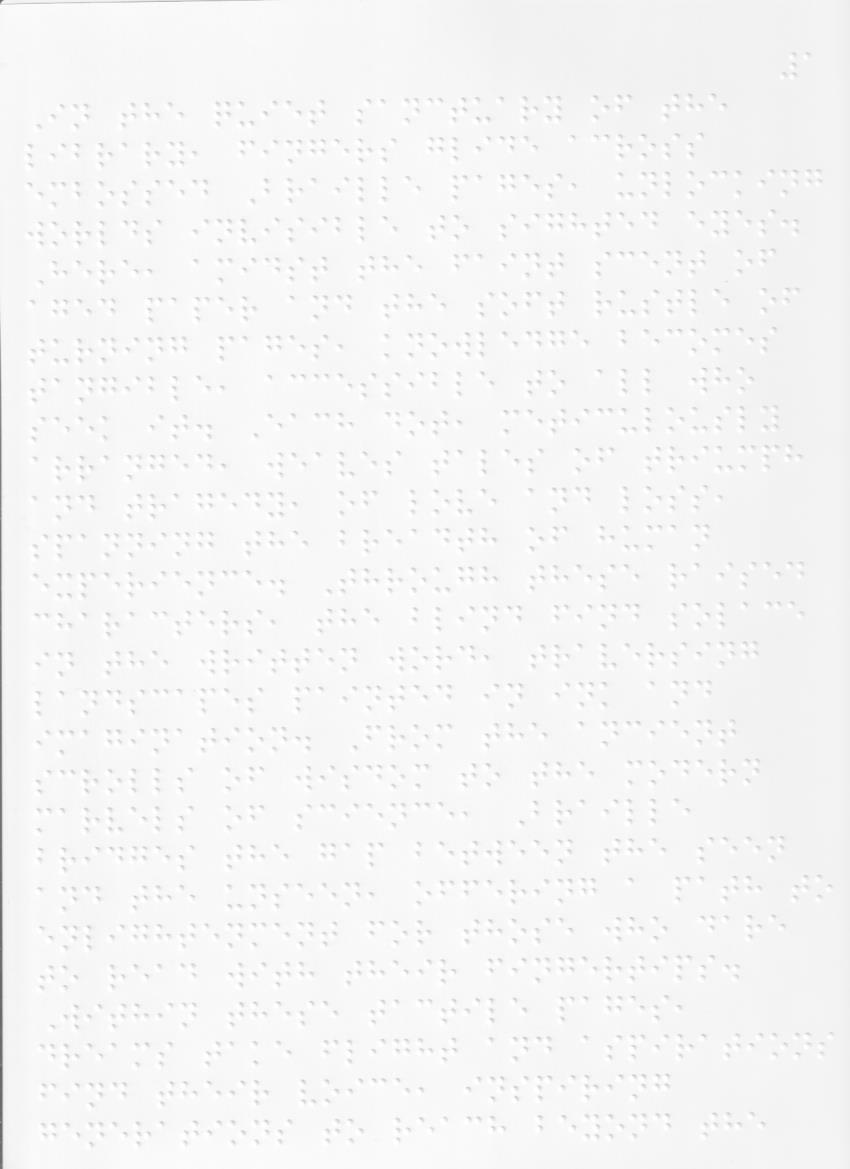
\includegraphics[width=0.5\linewidth]{Image (43).jpg}}
    \subfloat[the undetected dots in the page]{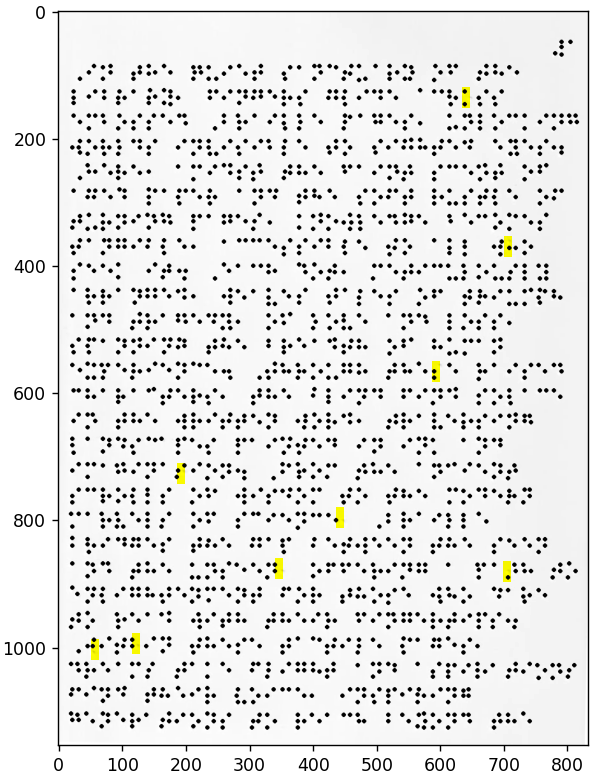
\includegraphics[width=0.5\linewidth]{ex22.PNG}}\hfill
  
    \caption{example of the Hough circle transformation used for dot detection }
    \label{fig:num2}
\end{figure}


\subsection{Image Processing Translation Results}
Although we use an AI model for character classification. Our Image Processing algorithm is capable of classifying characters after identifying them as mentioned, leading to a translation accuracy of 97.98\%.  (20 mistakes out of 989 words including punctuation) .This approach can be time efficient as AI classification can be difficult and resource-consuming for some machines.

        \begin{figure}[h!]
            \centering
            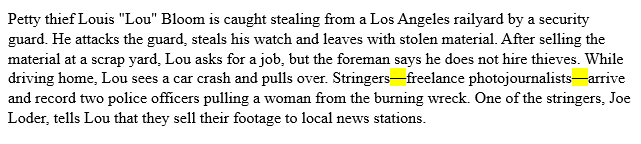
\includegraphics[width=0.6\textwidth]{ip.png}
            
            \caption{Image Processing Algorithm Translation: 2 Dashing Mistakes}
        \end{figure}

\subsection{AI Translation Results}
The AI-based translation step classifies the detected Braille characters into the corresponding text. This was tested using a pre-trained model on a diverse set of Braille samples. The AI model demonstrated a high classification accuracy on the test set of 99\%, correctly identifying the majority of the Braille characters.
When tested on 5 images the system gave 94.45\% accuracy. This was achieved by translating 5 wrong words out of 3.



\subsection{Text Correction Results}
Following the AI translation, the text correction step was applied to improve the accuracy of the translated text. This step is crucial as it involves correcting any misclassifications and ensuring that the corrected text adheres to grammatical and syntactical standards while maintaining the context of the translated passage. For this task, we employed the AI Forever T5 spell checker, a model renowned for its robust performance in text correction tasks.

The AI Forever T5 spell checker, which is based on the T5 (Text-To-Text Transfer Transformer) architecture, has shown exceptional capabilities in handling text correction due to its extensive pre-training on a diverse corpus and its sophisticated sequence-to-sequence learning mechanism. This model outperforms previous generation models like GPT-3.5 in several benchmarks, particularly in tasks requiring precise grammatical corrections and context preservation. Further details about the AI Forever T5 model can be found in Chapter 7, Section 2.

In our application, the text correction process achieved an impressive accuracy of 100\%, largely due to the high accuracy of the initial translation step, which minimized the number of errors needing correction. While the AI Forever T5 model has a reported overall accuracy of 83\% in general text correction tasks, our specific use case involved small paragraphs with a limited number of misspelled words. This controlled scenario allowed the model to perform with significantly higher accuracy. The effectiveness of the AI Forever T5 spell checker in our context underscores its capability to handle nuanced and context-sensitive text correction tasks with high precision, making it a valuable tool in our translation and text correction pipeline. The following are some additional example outputs.



\subsubsection*{Example 1}
\begin{itemize}
    \item \textbf{Original Passage}: \textcolor{red}{Th} \textcolor{red}{quikc} \textcolor{red}{borwn} fox \textcolor{red}{jmups} \textcolor{red}{ovre} the \textcolor{red}{lazi} dog.
    \item \textbf{Corrected Passage}: \uline{\textcolor{green}{The}} \uline{\textcolor{green}{quick}} \uline{\textcolor{green}{brown}} fox \uline{\textcolor{green}{jumps}} \uline{\textcolor{green}{over}} the \textcolor{green}{lazy} dog.
    \item \textbf{Misspelled Words}: 6
    \item \textbf{Corrected Words}: 6
    \item \textbf{Accuracy}: 100\%
\end{itemize}

\subsubsection*{Example 2}
\begin{itemize}
    \item \textbf{Original Passage}: I \textcolor{red}{cnnot} \textcolor{red}{beleive} how \textcolor{red}{beautifull} the \textcolor{red}{scenry}is at the \textcolor{red}{moountain.}
    \item \textbf{Corrected Passage}: I \uline{\textcolor{green}{cannot}} \uline{\textcolor{green}{believe}} how \uline{\textcolor{green}{beautiful}} the \uline{\textcolor{green}{scenery}} is at the \uline{\textcolor{green}{mountain.}}
    \item \textbf{Misspelled Words}: 5
    \item \textbf{Corrected Words}: 5
    \item \textbf{Accuracy}: 100\%
\end{itemize}

\subsubsection*{Example 3}
\begin{itemize}
    \item \textbf{Original Passage}: \textcolor{red}{Plase} \textcolor{red}{remmber} to bring \textcolor{red}{yoor} \textcolor{red}{umberela} \textcolor{red}{tomorow} \textcolor{red}{becase} it will rain.
    \item \textbf{Corrected Passage}: \uline{\textcolor{green}{Please}} \uline{\textcolor{green}{remember}} to bring \uline{\textcolor{green}{your}} \uline{\textcolor{green}{umbrella}} \uline{\textcolor{green}{tomorrow}} \uline{\textcolor{green}{because}} it will rain.
    \item \textbf{Misspelled Words}: 6
    \item \textbf{Corrected Words}: 6
    \item \textbf{Accuracy}: 100\%
\end{itemize}




\subsection{Overall Accuracy}
The overall accuracy of the Optical Braille Translator application was evaluated by combining the results of image processing, AI translation, and text correction. The performance metrics for each step and the cumulative accuracy are presented in the table below.

\begin{table}[h!]
    \centering
    \begin{tabular}{|l|c|}
        \hline
        \textbf{Process} & \textbf{Accuracy (\%)} \\
        \hline
        Detecting dots by image processing & 99.8\% \\
        \hline
        Classification of characters using AI model & 99\% \\
         \hline
        Word translation accuracy (Image Processing Algorithm) & 97.98\% \\
        \hline
        Word translation accuracy (AI Model) & 94.45\%\\
       
        \hline
        Correction accuracy & 100\% \\
        \hline
       
    \end{tabular}
    \caption{Accuracy results for different steps of the Optical Braille Translator application}
\end {table}

\subsection{Translation Speed}
The benefit of using image processing is most obvious when observing the speed of the different processes.  the system can finish all the image processing steps in under 1 second.  This includes filters, dot detection, grid formation, or white spaces detection  technique.  for example, one full page as an input scanned image to an output of non-corrected text takes 0.7 seconds to be processed.
On the other hand, AI models are not as fat because, as previously mentioned, they are resource-consuming and their performance varies from one machine to another.

\begin{table}[h!]
    \centering 
    \begin{tabular}{|l|p{3cm}|p{3cm}|p{3cm}|}
        \hline
        \textbf{User} & \textbf{Text Generation (seconds)} & \textbf{Text Correction (seconds)} & \textbf{Total Time (seconds)} \\
        \hline
        HP ProBook & 180 & 150 & 330 \\
        \hline
        Google Colab & 153 & 49 & 202 \\
        \hline
        Kaggle & 130 & 38 & 168 \\
        \hline
        ASUS TUF Gaming F17 & 91 & 30 & 121 \\
        \hline
    \end{tabular}
    \caption{Translation time for multiple users for one braille page}
    \label{tab:translation-times}
\end{table}